\documentclass{article}
\usepackage{graphicx} % Required for the inclusion of images
\usepackage{listings}
\usepackage{setspace}
\usepackage{geometry}
\usepackage{xcolor}
\usepackage{amsmath} % Required for some math elements 
\setlength\parindent{20pt} % Removes all indentation from paragraphs

\renewcommand{\labelenumi}{\alph{enumi}.} % Make numbering in the enumerate environment by letter rather than number (e.g. section 6)
\renewcommand{\baselinestretch}{1.25}
%\usepackage{times} % Uncomment to use the Times New Roman font

\newgeometry{top=2.3cm}

\title{Lab 3 Web Development \\ EE 101} 
\author{Lifan Zhang} 
\date{2019.5.15} 
\begin{document}

\maketitle 
% \begin{abstract}
% Abstract text
% \end{abstract}

\section{Data Processing}
\hspace*{0.5cm}
The aim of our project \emph{PaperHub} is to show the visitors the data about the papers, authors, affiliations and
other academic units, so as the basis of the project, we need to do some data processing first. First we want to score
the authors according to the citations of his or her papers, and his or her rank of authors in the papers. The maximum 
number of authers is 57 in the data provided by the teaching assistant of EE101, so we design a function to weight the 
academic achievement of the author. Then we calculate the score of each author and affiliation, and write it into two
new tables in our MySQL database.

\begin{figure}[h]
\begin{center}
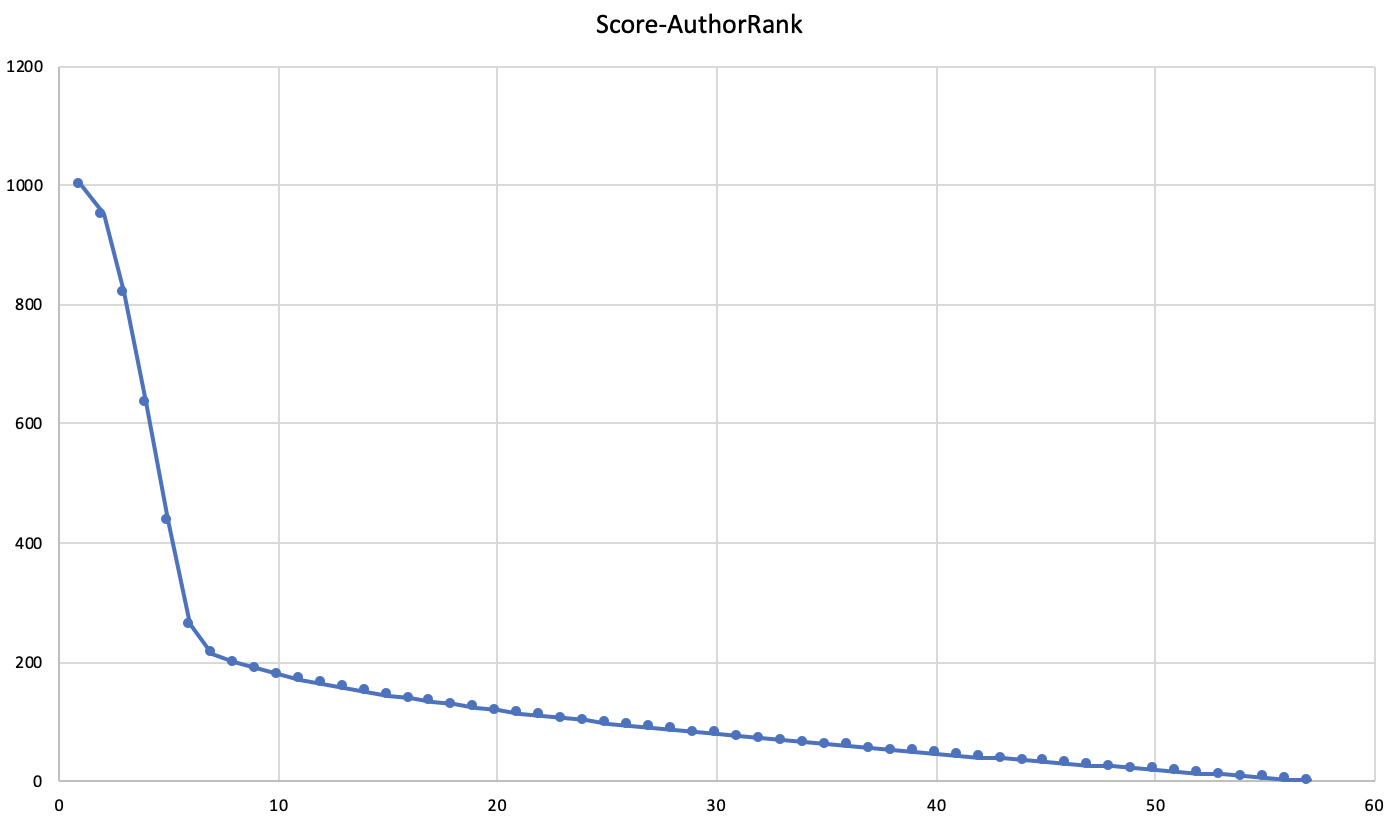
\includegraphics[width=0.95\textwidth]{zlf_1} % Include the image placeholder.png
\caption{The score range from 2 to 1000}
\end{center}
\end{figure}

\section{Website Deployment}
\hspace*{0.5cm}
First we buy a domain and an ECS Server from Aliyun and install Ubuntu 18.04. Then we use apt command to install python,
MySQL, Nginx, PHP and other essential software. After uploading our website to the server through SFTP, we add a server 
into the configuration of Nginx to let it listen port 80 on the domain acemap.lifanz.cn. To make our website legal, we 
registered it to MIIT and the public security department, to get an ICP registration number and a public security 
registration number. Finally, we use certbot the enable SSL connection throught port 443.

\begin{figure}[h]
\begin{center}
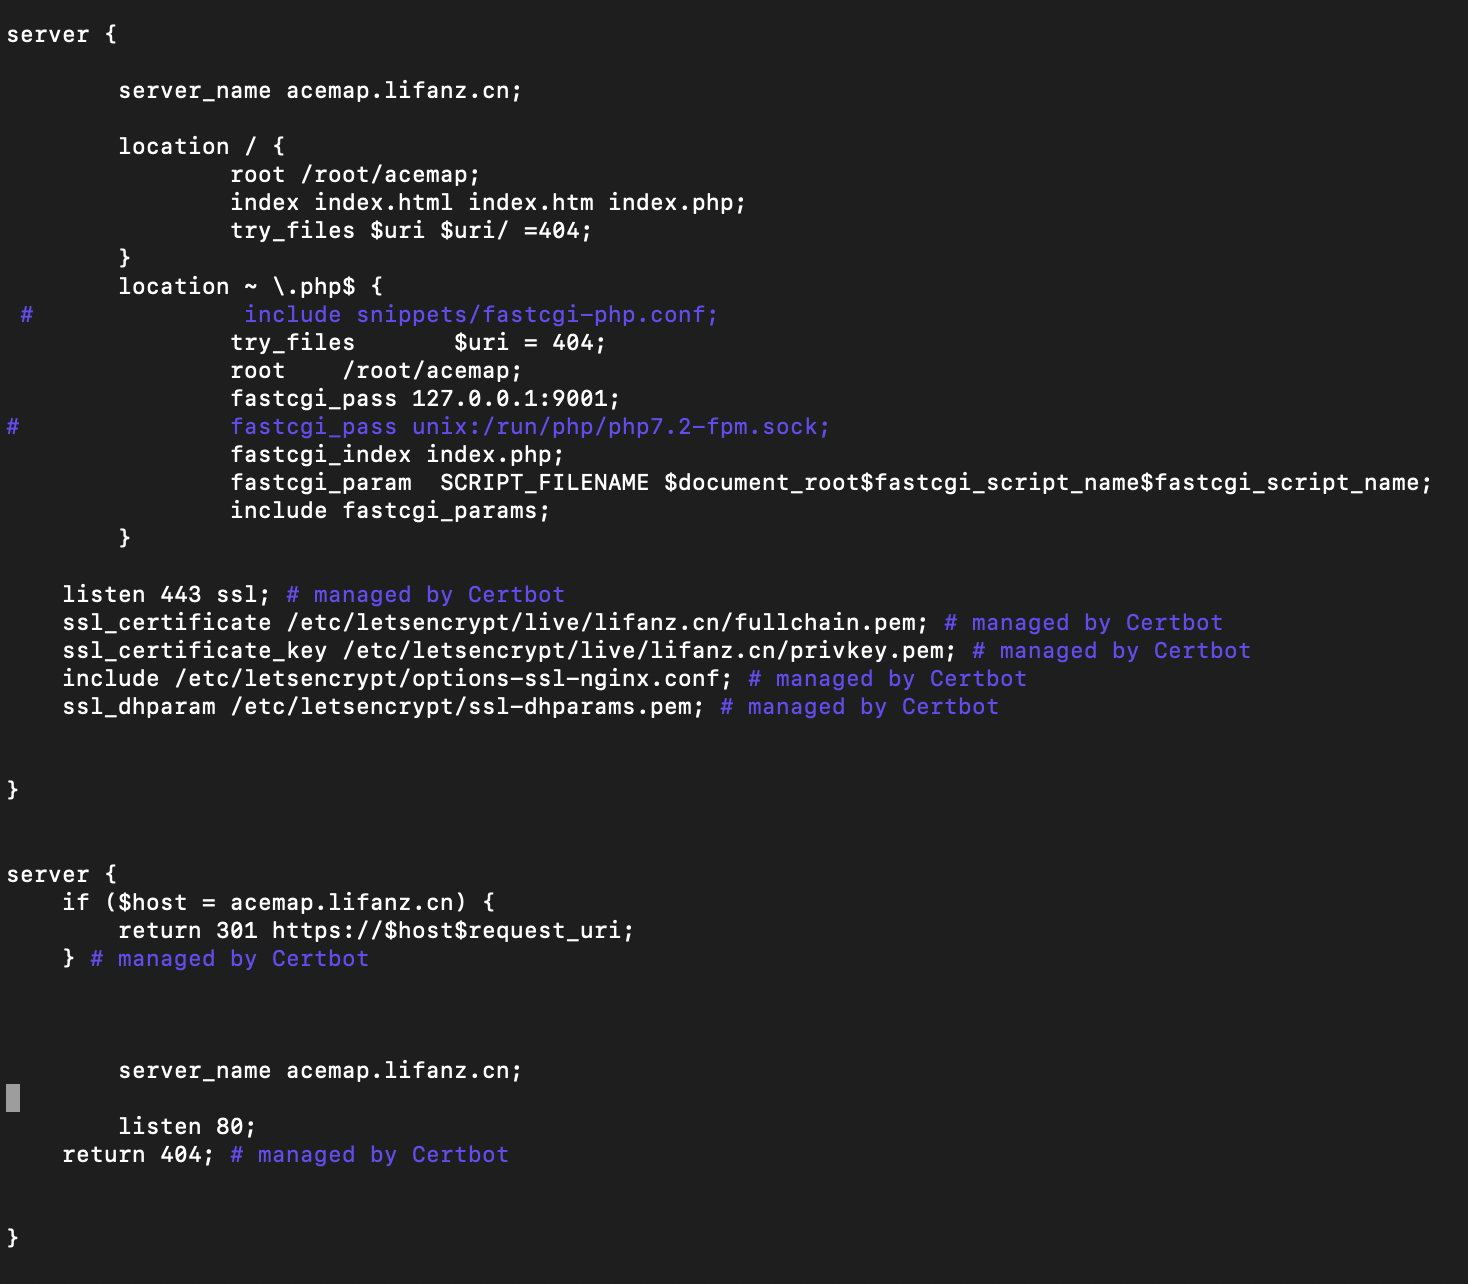
\includegraphics[width=0.95\textwidth]{zlf_2} % Include the image placeholder.png
\caption{The configuration of Nginx}
\end{center}
\end{figure}

\section{Homepage}
\hspace*{0.5cm}
In the homepage, we want to realize two functions. The first one is a general searching input box. In the box, the user
can search everything he want, and the webpage will guess what the user want to search and give the user some hints in a
dropdown list. The second one is an advanced search form, where the user can specify the type of data he want to get.
We use bootstrap and a model(https://github.com/BlackrockDigital/startbootstrap) to beautify the homepage.\\
To realize realtime search suggestion, we built a new solr core, which includes the papers of lots of citations and is much
smaller than the former one, because if we use the former core, it will take too much time to search. And we need to make
a search operation when the user press a key on the keyboard, if it is too slow, the experience of the user will be stuck.
The solr core returns a json array to the homepage, and the homepage will show it in a droplist.

\begin{figure}[h]
\begin{center}
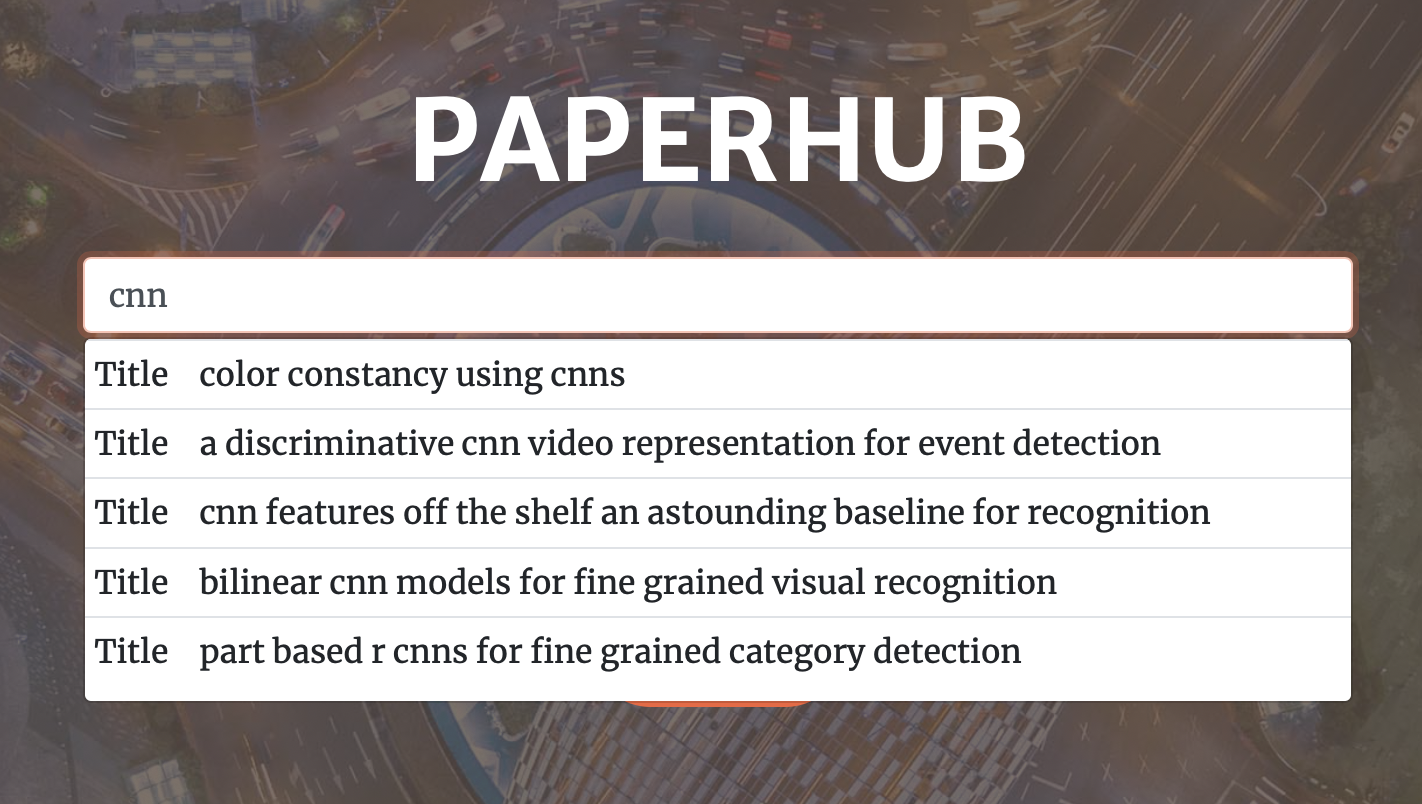
\includegraphics[width=0.92\textwidth]{zlf_3} % Include the image placeholder.png
\caption{The search suggestion droplist}
\end{center}
\end{figure}

\end{document}

